% Options for packages loaded elsewhere
\PassOptionsToPackage{unicode}{hyperref}
\PassOptionsToPackage{hyphens}{url}
%
\documentclass[
]{book}
\usepackage{lmodern}
\usepackage{amssymb,amsmath}
\usepackage{ifxetex,ifluatex}
\ifnum 0\ifxetex 1\fi\ifluatex 1\fi=0 % if pdftex
  \usepackage[T1]{fontenc}
  \usepackage[utf8]{inputenc}
  \usepackage{textcomp} % provide euro and other symbols
\else % if luatex or xetex
  \usepackage{unicode-math}
  \defaultfontfeatures{Scale=MatchLowercase}
  \defaultfontfeatures[\rmfamily]{Ligatures=TeX,Scale=1}
\fi
% Use upquote if available, for straight quotes in verbatim environments
\IfFileExists{upquote.sty}{\usepackage{upquote}}{}
\IfFileExists{microtype.sty}{% use microtype if available
  \usepackage[]{microtype}
  \UseMicrotypeSet[protrusion]{basicmath} % disable protrusion for tt fonts
}{}
\makeatletter
\@ifundefined{KOMAClassName}{% if non-KOMA class
  \IfFileExists{parskip.sty}{%
    \usepackage{parskip}
  }{% else
    \setlength{\parindent}{0pt}
    \setlength{\parskip}{6pt plus 2pt minus 1pt}}
}{% if KOMA class
  \KOMAoptions{parskip=half}}
\makeatother
\usepackage{xcolor}
\IfFileExists{xurl.sty}{\usepackage{xurl}}{} % add URL line breaks if available
\IfFileExists{bookmark.sty}{\usepackage{bookmark}}{\usepackage{hyperref}}
\hypersetup{
  pdftitle={Lecture Notes},
  pdfauthor={Author Name Goes Here},
  hidelinks,
  pdfcreator={LaTeX via pandoc}}
\urlstyle{same} % disable monospaced font for URLs
\usepackage[margin=1in]{geometry}
\usepackage{color}
\usepackage{fancyvrb}
\newcommand{\VerbBar}{|}
\newcommand{\VERB}{\Verb[commandchars=\\\{\}]}
\DefineVerbatimEnvironment{Highlighting}{Verbatim}{commandchars=\\\{\}}
% Add ',fontsize=\small' for more characters per line
\usepackage{framed}
\definecolor{shadecolor}{RGB}{248,248,248}
\newenvironment{Shaded}{\begin{snugshade}}{\end{snugshade}}
\newcommand{\AlertTok}[1]{\textcolor[rgb]{0.94,0.16,0.16}{#1}}
\newcommand{\AnnotationTok}[1]{\textcolor[rgb]{0.56,0.35,0.01}{\textbf{\textit{#1}}}}
\newcommand{\AttributeTok}[1]{\textcolor[rgb]{0.77,0.63,0.00}{#1}}
\newcommand{\BaseNTok}[1]{\textcolor[rgb]{0.00,0.00,0.81}{#1}}
\newcommand{\BuiltInTok}[1]{#1}
\newcommand{\CharTok}[1]{\textcolor[rgb]{0.31,0.60,0.02}{#1}}
\newcommand{\CommentTok}[1]{\textcolor[rgb]{0.56,0.35,0.01}{\textit{#1}}}
\newcommand{\CommentVarTok}[1]{\textcolor[rgb]{0.56,0.35,0.01}{\textbf{\textit{#1}}}}
\newcommand{\ConstantTok}[1]{\textcolor[rgb]{0.00,0.00,0.00}{#1}}
\newcommand{\ControlFlowTok}[1]{\textcolor[rgb]{0.13,0.29,0.53}{\textbf{#1}}}
\newcommand{\DataTypeTok}[1]{\textcolor[rgb]{0.13,0.29,0.53}{#1}}
\newcommand{\DecValTok}[1]{\textcolor[rgb]{0.00,0.00,0.81}{#1}}
\newcommand{\DocumentationTok}[1]{\textcolor[rgb]{0.56,0.35,0.01}{\textbf{\textit{#1}}}}
\newcommand{\ErrorTok}[1]{\textcolor[rgb]{0.64,0.00,0.00}{\textbf{#1}}}
\newcommand{\ExtensionTok}[1]{#1}
\newcommand{\FloatTok}[1]{\textcolor[rgb]{0.00,0.00,0.81}{#1}}
\newcommand{\FunctionTok}[1]{\textcolor[rgb]{0.00,0.00,0.00}{#1}}
\newcommand{\ImportTok}[1]{#1}
\newcommand{\InformationTok}[1]{\textcolor[rgb]{0.56,0.35,0.01}{\textbf{\textit{#1}}}}
\newcommand{\KeywordTok}[1]{\textcolor[rgb]{0.13,0.29,0.53}{\textbf{#1}}}
\newcommand{\NormalTok}[1]{#1}
\newcommand{\OperatorTok}[1]{\textcolor[rgb]{0.81,0.36,0.00}{\textbf{#1}}}
\newcommand{\OtherTok}[1]{\textcolor[rgb]{0.56,0.35,0.01}{#1}}
\newcommand{\PreprocessorTok}[1]{\textcolor[rgb]{0.56,0.35,0.01}{\textit{#1}}}
\newcommand{\RegionMarkerTok}[1]{#1}
\newcommand{\SpecialCharTok}[1]{\textcolor[rgb]{0.00,0.00,0.00}{#1}}
\newcommand{\SpecialStringTok}[1]{\textcolor[rgb]{0.31,0.60,0.02}{#1}}
\newcommand{\StringTok}[1]{\textcolor[rgb]{0.31,0.60,0.02}{#1}}
\newcommand{\VariableTok}[1]{\textcolor[rgb]{0.00,0.00,0.00}{#1}}
\newcommand{\VerbatimStringTok}[1]{\textcolor[rgb]{0.31,0.60,0.02}{#1}}
\newcommand{\WarningTok}[1]{\textcolor[rgb]{0.56,0.35,0.01}{\textbf{\textit{#1}}}}
\usepackage{longtable,booktabs}
% Correct order of tables after \paragraph or \subparagraph
\usepackage{etoolbox}
\makeatletter
\patchcmd\longtable{\par}{\if@noskipsec\mbox{}\fi\par}{}{}
\makeatother
% Allow footnotes in longtable head/foot
\IfFileExists{footnotehyper.sty}{\usepackage{footnotehyper}}{\usepackage{footnote}}
\makesavenoteenv{longtable}
\setlength{\emergencystretch}{3em} % prevent overfull lines
\providecommand{\tightlist}{%
  \setlength{\itemsep}{0pt}\setlength{\parskip}{0pt}}
\setcounter{secnumdepth}{5}
% preamble for book
\usepackage{color}
\usepackage{ifthen}
\usepackage{geometry}
\usepackage{geometry}
%\usepackage[top=2cm, bottom=1.3cm, left=5cm, right=0.5cm, heightrounded,
%  marginparwidth=4.6cm, marginparsep=3mm]{geometry}
\usepackage{marginnote}
\usepackage{float}
\usepackage{graphicx}
\usepackage{subfig}
\usepackage{xcolor}
\usepackage{framed}

% mdframed
%\usepackage{mdframed}
\usepackage[framemethod=tikz]{mdframed}
\mdfsetup{skipabove=2pt,skipbelow=5pt}

\mdfdefinestyle{myframestyle}{%
    outerlinewidth=0.1pt
}

\newcommand{\proglang}[1]{\textsf{#1}}
\newcommand{\pkg}[1]{\textbf{#1}}
\newcommand{\faq}[1]{FAQ~\ref{#1}}
\newcommand{\dd}{\mathrm{d}}

% takes care of gaps
% to modify the boolean, needs to be passed from makeRmd.R
\newboolean{gaptextisblue}
\setboolean{gaptextisblue}{true} 

% to modify the boolean, needs to be passed from makeRmd.R
\newboolean{useframe}
\setboolean{useframe}{true}

\newboolean{showtext}
\setboolean{showtext}{true} 

\newboolean{showsidenotes}
\setboolean{showsidenotes}{true} 


\newboolean{moreboxspace}
\setboolean{moreboxspace}{true} 

\newcommand{\makeblank}[1]{ \vphantom{#1} }
\newcommand{\makeblue}[1]{\textcolor{blue}{#1}}
\newcommand{\makered}[1]{\textcolor{red}{#1}}
\newcommand{\makenormalcolour}[1]{#1}

% text in gaps:
\newcommand{\gaptext}{\ifthenelse{\boolean{gaptextisblue}}{\makeblue}{\makenormalcolour}}

% to be or not to be - controls the display of gappy text
\newcommand{\tbontb}{\ifthenelse{\boolean{showtext}}{\gaptext}{\makeblank}}

% notes in the margin
%https://tex.stackexchange.com/questions/29125/how-to-get-marginnote-to-use-the-whole-margin-space
\newcommand{\makemarginnote}[1]{\marginnote{\footnotesize\makeblue{#1}}}
\newcommand{\sidenote}{\ifthenelse{\boolean{showsidenotes}}{\makemarginnote}{}}
\setlength{\marginparwidth}{1.7cm}


% Add box space
\newcommand{\addboxspace}{\vspace{0.2cm}}
\newcommand{\maybeaddboxspace}{\ifthenelse{\boolean{moreboxspace}}{\addboxspace}{}}


% framed equation
\newenvironment{fequation}
    {\ifthenelse{\boolean{useframe}}{\begin{mdframed}[style=myframestyle]}{}
    \maybeaddboxspace
    \begin{equation}
        }
        {
    \end{equation} 
    \maybeaddboxspace
    \ifthenelse{\boolean{useframe}}{\end{mdframed}}{}
    }

% general framebox for text/align
\newenvironment{ftext}
    {\ifthenelse{\boolean{useframe}}{\begin{mdframed}[style=myframestyle]}{}
        }
        {
    \ifthenelse{\boolean{useframe}}{\end{mdframed}}{}
    }


%%=========================================================================%%
%% Changing the code colour scheme
%%=========================================================================%%
%\newcommand{\AlertTok}[1]{\textcolor[rgb]{0.94,0.16,0.16}{#1}}
%\newcommand{\AnnotationTok}[1]{\textcolor[rgb]{0.56,0.35,0.01}{\textbf{\textit{#1}}}}

%% Don't know
%\newcommand{\AttributeTok}[1]{\textcolor[rgb]{0.77,0.63,0.00}{#1}}
%\newcommand{\BaseNTok}[1]{\textcolor[rgb]{0.00,0.00,0.81}{#1}}
%\newcommand{\BuiltInTok}[1]{#1}

%% Not sure
%\newcommand{\CharTok}[1]{\textcolor[rgb]{0.31,0.60,0.02}{#1}}

%% Comment
%\newcommand{\CommentTok}[1]{\textcolor[rgb]{0.56,0.35,0.01}{\textit{#1}}}

%\newcommand{\CommentVarTok}[1]{\textcolor[rgb]{0.56,0.35,0.01}{\textbf{\textit{#1}}}}
%\newcommand{\ConstantTok}[1]{\textcolor[rgb]{0.00,0.00,0.00}{#1}}
%\newcommand{\ControlFlowTok}[1]{\textcolor[rgb]{0.13,0.29,0.53}{\textbf{#1}}}
%\newcommand{\DataTypeTok}[1]{\textcolor[rgb]{0.13,0.29,0.53}{#1}}
%\newcommand{\DecValTok}[1]{\textcolor[rgb]{0.00,0.00,0.81}{#1}}
%\newcommand{\DocumentationTok}[1]{\textcolor[rgb]{0.56,0.35,0.01}{\textbf{\textit{#1}}}}
%\newcommand{\ErrorTok}[1]{\textcolor[rgb]{0.64,0.00,0.00}{\textbf{#1}}}
%\newcommand{\ExtensionTok}[1]{#1}
%\newcommand{\FloatTok}[1]{\textcolor[rgb]{0.00,0.00,0.81}{#1}}

%% R Functions actually seem to be keywords
%\newcommand{\FunctionTok}[1]{\textcolor[rgb]{0.00,0.00,0.00}{#1}}
%\newcommand{\ImportTok}[1]{#1}
%\newcommand{\InformationTok}[1]{\textcolor[rgb]{0.56,0.35,0.01}{\textbf{\textit{#1}}}}

%% These include functions such as rgamma
%\newcommand{\KeywordTok}[1]{\textcolor[rgb]{0.13,0.29,0.53}{\textbf{#1}}}

%\newcommand{\NormalTok}[1]{#1}
%\newcommand{\OperatorTok}[1]{\textcolor[rgb]{0.81,0.36,0.00}{\textbf{#1}}}
%\newcommand{\OtherTok}[1]{\textcolor[rgb]{0.56,0.35,0.01}{#1}}
%\newcommand{\PreprocessorTok}[1]{\textcolor[rgb]{0.56,0.35,0.01}{\textit{#1}}}
%\newcommand{\RegionMarkerTok}[1]{#1}
%\newcommand{\SpecialCharTok}[1]{\textcolor[rgb]{0.00,0.00,0.00}{#1}}
%\newcommand{\SpecialStringTok}[1]{\textcolor[rgb]{0.31,0.60,0.02}{#1}}
%%=========================================================================%%

%% Strings
%\newcommand{\StringTok}[1]{\textcolor[rgb]{0.31,0.60,0.02}{#1}}
    
%\newcommand{\VariableTok}[1]{\textcolor[rgb]{0.00,0.00,0.00}{#1}}
%\newcommand{\VerbatimStringTok}[1]{\textcolor[rgb]{0.31,0.60,0.02}{#1}}
%\newcommand{\WarningTok}[1]{\textcolor[rgb]{0.56,0.35,0.01}{\textbf{\textit{#1}}}}

%% Change comments to dark grey (black is (0,0,0))
\renewcommand{\CommentTok}[1]{\textcolor[rgb]{0.3,0.3,0.3}{\textit{#1}}}
%% Brown, but not italics
%\renewcommand{\CommentTok}[1]{\textcolor[rgb]{0.56,0.35,0.01}{#1}}

%\renewcommand{\KeywordTok}[1]{\textcolor[rgb]{0,0,0}{\textbf{#1}}}

%% FFAFFF, NiceLightPurple, 255, 175, 255
%\renewcommand{\KeywordTok}[1]{\textcolor[RGB]{255,175,255}{\textbf{#1}}}

%\renewcommand{\FunctionTok}[1]{\textcolor[rgb]{0,0,0}{\textbf{#1}}}
%\newcommand{\FunctionTok}[1]{\textcolor[rgb]{0.00,0.00,0.00}{#1}}

%% Make string bold
%\renewcommand{\StringTok}[1]{\textcolor[rgb]{0.31,0.60,0.02}{\textbf{#1}}}

%% Make string ArrowGreen
% 87FF87, RGB = 135, 255, 135
%\renewcommand{\StringTok}[1]{\textcolor[RGB]{135,255,135}{\textbf{#1}}}
%\renewcommand{\StringTok}[1]{\textcolor[RGB]{135,255,135}{#1}}


%% Make numbers orange
%% Hex E5786D
\renewcommand{\DecValTok}[1]{\textcolor[RGB]{229,120,109}{#1}}
%% Hex CB4B16
\renewcommand{\DecValTok}[1]{\textcolor[RGB]{203,75,22}{#1}}

% framed align
% will not work,  need to do manually
%\newenvironment{ffalign}
%    {\ifthenelse{\boolean{useframe}}{\begin{mdframed}}{}
%    \begin{align}
%        }
%        {
%    \end{align} 
%    \ifthenelse{\boolean{useframe}}{\end{mdframed}}{}
%    }
\usepackage[]{natbib}
\bibliographystyle{apalike}

\title{Lecture Notes}
\author{Author Name Goes Here}
\date{2019-08-26}

\begin{document}
\frontmatter
\maketitle

{
\setcounter{tocdepth}{2}
\tableofcontents
}
\mainmatter
\setboolean{showtext}{true}
\setboolean{useframe}{true}
\setboolean{gaptextisblue}{true}
\setboolean{showsidenotes}{false}
\setboolean{moreboxspace}{false}
\renewcommand{\addboxspace}{\vspace{0.9cm}}

\definecolor{fancyTextColor}{HTML}{4284f5}
\definecolor{hightlightColor}{HTML}{FFFF66}

\hypertarget{distributions}{%
\chapter{Distributions}\label{distributions}}

\hypertarget{sec:getting-started}{%
\section{How do I get started}\label{sec:getting-started}}

The \proglang{R} package \pkg{xtable} is useful.
For a description of the bootstrap, see \citet{Efron1979Bootstrap}.
A good book is \citep{CLRS}.
This is Section \ref{sec:getting-started}.
Check \texttt{index.Rmd} to see which R packages are loaded.

\hypertarget{normal-distribution}{%
\section{Normal Distribution}\label{normal-distribution}}

The probability density function for the standard normal distribution is (blanked out):

\begin{fequation}
        \label{eqn:normpdf}
        \tbontb{
        f(x) = \frac{1}{\sqrt{2\pi}} \int_{-\infty}^{x} e^{-x^2}  \dd  x.
        % THIS IS COMMENTED OUT
        }
\end{fequation}

Equation \eqref{eqn:normpdf} is awesome.

Here is a plot of the probability density function of a standard normal:

\begin{center}\includegraphics{lecturenotes_gapfilled_files/figure-latex/normpdf-1} \end{center}

\hypertarget{gamma-distribution}{%
\section{Gamma distribution}\label{gamma-distribution}}

The gamma distribution has two parameters, shape \(k\) and scale \(\theta\), and is denoted \(\Gamma(k, \theta)\).
Data for a \(\Gamma(1, 2)\) distribution can be generated as follows:

\begin{Shaded}
\begin{Highlighting}[]
\CommentTok{# We set the seed here}
\KeywordTok{set.seed}\NormalTok{(}\DecValTok{1}\NormalTok{)}
\NormalTok{k <-}\StringTok{ }\DecValTok{1}
\NormalTok{ylab <-}\StringTok{  "Value"} \CommentTok{# set elsewhere}
\NormalTok{theta <-}\StringTok{ }\DecValTok{2}
\NormalTok{x <-}\StringTok{ }\KeywordTok{rgamma}\NormalTok{(}\DecValTok{10}\NormalTok{, }\DataTypeTok{shape=}\NormalTok{k, }\DataTypeTok{scale=}\NormalTok{theta)}
\KeywordTok{print}\NormalTok{(x)}
\CommentTok{#>  [1] 0.31028 3.76480 3.60902 1.67236 2.44509 2.31671 1.98004}
\CommentTok{#>  [8] 0.61475 0.18924 0.31440}
\end{Highlighting}
\end{Shaded}

And here is the data plotted in Figure \ref{fig:gammadataplot}:

\begin{figure}[H]

{\centering \includegraphics{lecturenotes_gapfilled_files/figure-latex/gammadataplot-1} 

}

\caption{Gamma data for $\Gamma(1, 2)$}\label{fig:gammadataplot}
\end{figure}

Figure \ref{fig:gammadataplot} should be above this line.

\clearpage

\hypertarget{cars}{%
\section{Cars}\label{cars}}

Here is some \texttt{cars} data:

\begin{figure}[H]

{\centering \subfloat[A figure caption\label{fig:carsfigureandtable1}]{\includegraphics[width=.49\linewidth]{lecturenotes_gapfilled_files/figure-latex/carsfigureandtable-1} }\subfloat[A table caption\label{fig:carsfigureandtable2}]{\includegraphics[width=.49\linewidth]{lecturenotes_gapfilled_files/figure-latex/carsfigureandtable-2} }

}

\caption{Caption text for Figure and Table}\label{fig:carsfigureandtable}
\end{figure}

Look at Figure \ref{fig:carsfigureandtable}, it contains a figure (a) and a table (b).

Here is a box of text, using \texttt{ftext} command:

\sidenote{Don't take the following too seriously.}
\begin{ftext}
\tbontb{
\begin{minipage}{\textwidth}
There are three types of lies---lies, damn lies, and statistics. 
There are three types of lies---lies, damn lies, and statistics
There are three types of lies---lies, damn lies, and statistics
There are three types of lies---lies, damn lies, and statistics
There are three types of lies---lies, damn lies, and statistics
\end{minipage}
}
\end{ftext}

\sidenote{See the code for this `align` example for an example
of creating a gapped `align`.}

Here is an aligned equation, need to use in \texttt{ftext}:

\begin{ftext}
    \begin{align}
        \tbontb{y}  & \tbontb{= 2} \label{eqn:blank} \\
        z &= 2 
    \end{align}
\end{ftext}

Equation \eqref{eqn:blank} is blank in an align environment.

Using \texttt{fequation}:

\begin{fequation}
t = 1
\end{fequation}

It might be useful to include notes on the side, in the margin. These can be done using \texttt{sidenote}.
\sidenote{Here is an example of a sidenote}
And more text goes here, and one can read the note in the margin to remember certain points.

\clearpage

\hypertarget{tikz-figures}{%
\section{tikz figures}\label{tikz-figures}}

Here is a figure created using \texttt{tikz}, which creates an intermediate tex and pdf.

\begin{figure}[H]

{\centering 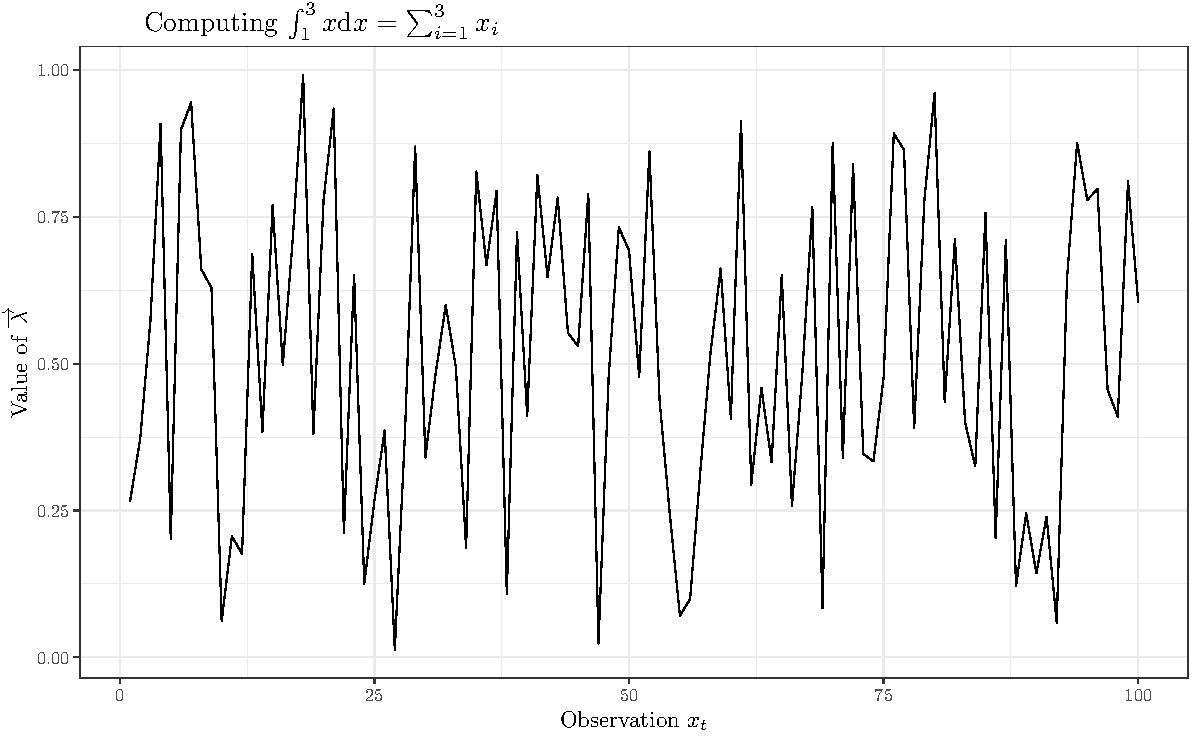
\includegraphics[width=0.9\linewidth]{Rcode/tikzfig} 

}

\caption{Caption for tikz figure showing $\overrightarrow{\lambda}$, and with a sum $\sum_{i=1}^{3} x_i$.}\label{fig:unnamed-chunk-1}
\end{figure}

\backmatter
  \bibliography{refs.bib}

\end{document}
